
\documentclass[11pt]{article}
\usepackage[a4paper, hmargin={2.8cm, 2.8cm}, vmargin={2.5cm, 2.5cm}]{geometry}
\usepackage{eso-pic} % \AddToShipoutPicture
\usepackage{graphicx} % \includegraPhics
\usepackage{placeins}
\usepackage{amsmath} % flere matematikkommandoer
\usepackage[utf8]{inputenc} % æøå
\usepackage[T1]{fontenc} % mere æøå
\usepackage{verbatim} % så man kan skrive ren tekst
\usepackage[all]{xy} % den sidste (avancerede) formel i dokumentet
\usepackage{amssymb}
\usepackage{listings}
\usepackage{hyperref}
\usepackage{multicol}
\usepackage{color}
\usepackage{url}
\usepackage{tcolorbox}
\usepackage{enumerate}
\usepackage{caption}
\usepackage{subcaption}
\usepackage{float}
\usepackage{glossaries}
\usepackage{pdflscape}

\newacronym{POS}{POS}{Parts-of-Speech}
\newacronym{ISG}{ISG}{Integrated Syntactic Graph}
\newacronym{UBM}{UBM}{Universal Background Model}
\newacronym{AGS}{AGS}{Average Group Similarity}
\newacronym{AUC}{AUC}{Area Under the Curve}
\newacronym{SCAP}{SCAP}{Source Code Author Profile}
\newacronym{CNG}{CNG}{Common n-gram}
\newacronym{LNG}{LNG}{Local n-gram}
\newacronym{RLP}{RLP}{Recentred Local Profiles}
\newacronym{KNN}{KNN}{K-Nearest Neighbours}
\newacronym{SVM}{SVM}{Support Vector Machine}
\newacronym{TPR}{TPR}{True Positive Rate}
\newacronym{TNR}{TNR}{True Negative Rate}

\author{
    \Large{August V. S\o rensen \& Magnus N\o rskov Stavngaard} \\
    \texttt{august.vinkel@gmail.com \& magnus@stavngaard.dk} \\
}

\title{
    \vspace{3cm}
    \Huge{Authorship Verification} \\
    \Large{Project Outside Course Scope}
}

\usepackage{fancyhdr}
\pagestyle{fancy}

\lhead{University of Copenhagen}
\rhead{August V. S\o rensen \& Magnus N\o rskov Stavngaard}
%\cfoot{}
%\rfoot{\thepage}

\begin{document}

    \AddToShipoutPicture*{\put(0,0){\includegraphics*[viewport=0 0 700 600]{include/ku-farve}}}
    \AddToShipoutPicture*{\put(0,602){\includegraphics*[viewport=0 600 700 1600]{include/ku-farve}}}
    \AddToShipoutPicture*{\put(0,0){\includegraphics*{include/ku-en}}}
    \clearpage\maketitle
    \thispagestyle{empty}
    \newpage

    \section{Abstract}


    \newpage
    \tableofcontents
    \newpage

    \section{Introduction}
Authorship verification is the process of verifying the authorship of a text.
You are given a set of texts known to be written by the author and an unknown
text that has to be classified as either written by the author or someone else.
The normal approach to the problem is to use stylometry to extract features from
the text and then some form of machine learning or statistical method to analyse
the data \cite{stamatos2009}. A lot of different text features has been proposed
as describing an authors writing style. That includes but is not limited to
character frequencies, word frequencies, vocabulary size, sentence length,
punctuation usage, character n-grams, word n-grams and \gls{POS} tagging n-grams
\cite{stamatos2009}.

Authorship verification has been used for plagiarism control in danish secondary
schools \cite{hansen2014} and also has uses in civil law, criminal law and
computer forensics \cite{stamatos2009}.

In this article we explore state of the art methods for authorship verification.
We extract several different types of features including word frequencies, word
n-grams and pos-tagging n-grams. We implement several different algorithms to
work on the features. We start by implementing a baseline method which is a
distance based approach where an unknown text is considered to be written by
the closest author. We then use the baseline method to compare to our other
results. We use data from two sources \cite{pan:2015} and \cite{pan:2013} which
are two instances of a yearly competition in digital text forensics. Since we
use PAN data we also compare our results to the results obtained by others in
the competition.

% TODO: Continue.
%The PAN2013 and PAN2015 datasets are very different. The PAN2013 dataset
%contains many texts from a few authors while the PAN2015 texts contains a single
%text from many authors.


    \section{Related Work}


    \section{Method} \label{sec:method}
In this section we will describe the methods we have implemented to solve the
PAN 2013 and PAN 2015 problems. The problems are both known as authorship
verification problems. \cite{stamatos2009} describes the problem in a machine
learning sense as a two class classification problem. Either the unknown texts
are written by the same author or they are written by different authors. All
our implemented methods solve that classification problem by answering either
\textit{True} (unknown text is written by the same author as the known texts) or
\textit{False} (unknown text is \textbf{not} written by the same author as the
known texts). Since both PAN 2013 and PAN 2015 is a binary decision problem we
can compute the number of \gls{TP}, \gls{TN}, \gls{FP} and \gls{FN}. In these
problems we get,

\begin{itemize}
    \item a \gls{TP} whenever we answer \textit{True} and the texts are written
        by the same author,
    \item a \gls{TN} whenever we answer \textit{False} and the texts are
        \textbf{not} written by the same author,
    \item a \gls{FP} whenever we answer \textit{True} and the texts are
        \textbf{not} written by the same author,
    \item a \gls{FN} whenever we answer \textit{False} and the texts are written
        by the same author.
\end{itemize}

Given those definitions the \gls{TPR}, \gls{FPR}, \gls{TNR} and \gls{FNR}
describes.

\begin{description}
    \item[\gls{TPR}: ] The fraction of positives that we reported \textit{True}
        on i.e. the fraction of texts written by the same author that we say are
        written by the same author.
    \item[\gls{FPR}: ] The fraction of negatives that we reported \textit{True}
        on i.e. the fraction of texts written by different authors that we say
        are written by the same author.
    \item[\gls{TNR}: ] The fraction of negatives that we reported \textit{False}
        on i.e. the fraction of texts written by different authors that we say
        are written by different authors.
    \item[\gls{FNR}: ] The fraction of positives that we reported \textit{False}
        on i.e. the fraction of texts written by the same author that we say are
        written by different authors.
\end{description}

And they can be computed as,

\begin{align}
    TPR &= \frac{TP}{TP + FN}, \\
    FPR &= \frac{FP}{FP + TN}, \\
    TNR &= \frac{TN}{TN + FP}, \\
    FNR &= \frac{FN}{FN + TP}.
\end{align}

\cite{stamatos2009} describes instance based and profile based approaches for
authorship attribution/verification. The instance based approach uses several
texts from an author to create multiple different feature vectors representing
the authors writing style while the profile based approach concatenates all
texts to a single text and creates only a single vector representing that text.
The instance based approach corresponds to the PAN 2013 problem. In that problem
we are given multiple texts to train from and the methods we have implemented to
solve that problem will reflect that property. The profile based approach
corresponds to the PAN 2015 dataset here we are given only a single known text
per author which we can use to construct a profile of the author.

\subsection{Text Features} \label{subsec:method:text_features} Feature
extraction from a text is the process of finding a vector that represents
the text. There are a lot of different features that can be extracted when
performing \gls{NLP}. These features can span a lot of different linguistic
layers, including but not limited to, layers such as the character layer, which
describes a text on the character level, and the phonetic layer which analyses a
text based on the phonetic alphabet. We use features spanning several of these
layers. Specifically we use some character level features, some word level
features and some \gls{POS} tagging features. In this section we will define the
different features we use. The specific features used in different experiments
will be described at length under those experiments.

N-grams are subsequences extracted from a sequence of tokens. For example,
3-grams are all subsequences of length three of a given sequence. Using
individual characters as tokens, all \textit{character 3-grams} of the string
"hello" are "hel", "ell" and "llo". We use several different types of n-grams
in different experiments including character n-grams, word n-grams, special
character n-grams and \gls{POS}-tagging n-grams. Word n-grams are subsequences
of words, special character n-grams are subsequences of characters with
alphanumeric and space characters removed and \gls{POS} tagging n-grams are
subsequences of \gls{POS} tags which are word classes such as noun, verbs and
adjectives. A special case of n-grams is 1-grams which is just a count of the
different tokens in a sequence. We will refer to 1-grams as frequencies.

\subsection{Delta Method} \label{subsec:method:delta_method}
We have chosen to use the Delta method as a baseline method for our other
implementations. The Delta method is described by \cite{evert2015towards} and
consist of extracting word frequencies, applying a linear transformation to
those frequencies and using \gls{KNN} with different distance metrics. There are
a number of parameters to choose. First of all the number of different words to
find frequencies for has to be chosen (it was originally chosen at 150 words
\cite{evert2015towards}). Then the linear transformation can be chosen, the
usual transformation is a normalization to zero mean unit variance. And finally
the distance metric can be chosen.

\subsection{Generalising Random Forest} \label{subsec:method:generalising_random_forest}
In addition to the delta method we chose to use the Random Forest approach
suggested by \cite{pacheco2015}. In our implementation we use different features
than in the their proposal. The idea of the method is to learn a general
difference between feature vectors of texts written by the same author and
feature vectors written by the different authors. The generalization is obtained
by combining the vectors of known texts with vectors of unknown text and
training on that combination instead of on the raw vectors. Rewriting the
encoding function used in \cite{pacheco2015}, we get the following combining
function,

\begin{equation}
    R_{i_k} = \frac{(A_{i_k}-U_{i_k})^2+1}{(B_k-U_{i_k})^2+1}
\end{equation}

Where $A$ is an author-specific text, $U$ is an author-unknown text, $B$ is a
\gls{UBM} describing a general author independent text. $i$ denotes from which
datapoint we get our author-specific and non-specific texts, and $k$ denotes a
specific feature of a given text. As such $R_{i_k}$ describes the encoding of a
specific feature for a specific data point.

The \gls{UBM} is meant to represent the features of an author independent
text. It is computed by concatenating all author-known-texts in the training
dataset and computing features from that resulting text. Since multiple authors
is then part of the text we are computing features from, the assumption is
that the author specific features will be averaged out and the \gls{UBM} will
represent the features of an author independent text. The addition of 1 in the
model prevent division by zero. Since 1 is added both in the numerator and the
denominator it does not otherwise change the result. The squaring of $(A_i -
U_i)$ and $(B - U_i)$ both prevent negative values and punishes values that are
far away. Therefore each value in the resulting encoded feature vector is in the
range $[0; \infty[$.

Let's examine what the above equation describes. Fix any specific $i$ and let
$A$ be $A_i$ and $U$ be $U_i$ then for each feature $k$ we compute,

\begin{equation}
\label{eq:rf-encode}
    R_k = \frac{(A_k-U_k)^2+1}{(B_k-U_k)^2+1},
\end{equation}

The $k$'th feature in each of the vectors is the same feature just extracted
from different texts. When the feature of the unknown text $U_k$ is closer to
$A_k$ than $B_k$ the numerator in the fraction will be greater than the
denominator giving us something in the range $[0; 1]$. When the feature of the
unknown text $U_k$ is closer to $B_k$ than $A_k$ the numerator will be lesser
than the denominator and we will therefore get a value in the interval
$[1; \infty[$. That results in $R$ being a vector containing values from 0 to
$\infty$ where it is between 0 and 1 whenever a feature is closer to the author
specific text than the universal text and greater than 1 otherwise.

The random forest algorithm is then trained on these encoded feature vectors
where it is supposed to learn a general difference between feature vectors of
the same author and feature vectors of different authors.

\subsection{Extended Delta} \label{subsec:method:extended_delta}
As described earlier there are many ways to extend and change the delta
method. We tried both using different features and different distance
measures to obtain better results than the Delta Method described in Section
\ref{subsec:method:delta_method}. The different feature combinations were tried
experimentally one after the other. If a feature combination did well on a
dataset we tried adding or removing features from that feature set to maybe
obtain something better. The features we tried were different combinations of
character n-grams, word n-grams and \gls{POS}-tag n-grams.

The different distance measures we tried were the Manhattan distance and the
Euclidean distance.

% TODO: Justify choices of distances.

\subsection{Author Specific SVM} \label{subsec:method:author_specific_svm}
We implemented an approach using \gls{SVM}'s inspired by \cite{hansen2014}. The
approach is only applicable to problems with more than a single text per author.
The classification in this approach is done by training an \gls{SVM} classifier
on all known texts of an author and an equal number of texts from other authors.
Then the unknown text is given to the \gls{SVM} and is classified either as
belonging to the same author or as belonging to a different author.

If there is only a single known text available for an author it does not make
sense to train an \gls{SVM} since there is simply too little data for it
to be a viable choice.

\subsection{Experiments} \label{subsec:method:experiments}
In this section we describe the different experiments we have performed.
We have tested the different methods we have implemented with different
features and on different datasets. In our experiments we use data from PAN
2013 \footnote{http://pan.webis.de/clef13/pan13-web/index.html} and PAN 2015
\footnote{http://pan.webis.de/clef15/pan15-web/index.html}.

The PAN 2013 data consist of texts from English, Greek and Spanish authors. We
work only on the English texts which consists of texts from 10 authors. For each
author there is (between 1 and 10) known texts and a single unknown text. The
task is, given the known texts of an author, to determine whether the unknown
text is written by the same author.

The PAN 2015 data consist of texts by authors in English, Dutch, Greek and
Spanish. Again we only work with English texts. Unlike the 2013 dataset there
is only a single known text for each author and a single unknown text. There
is therefore much less known data available for each author which makes the
verification harder. In the 2015 dataset there are 100 \textit{problems} in
which some of the known texts are the same (i.e. there are not 100 authors).

To generate metadata about English texts we use the Brown dataset
\footnote{http://clu.uni.no/icame/brown/bcm-los.html}. The brown dataset
contains more than 1,000,000 words across different genres and is therefore
perfect to use for our datasets. We specifically use the dataset to identify
the most frequently used n-grams (of all kinds). If we were to use our training
data to generate that we would risk having a bias towards our specific training
dataset.

We will evaluate the performance of the different algorithms on the training
data with the accuracy of the algorithms. The accuracy is computed as the number
of correct answers divided by the total number of problems. For some methods
we will also report the \gls{TPR} and \gls{TNR}, in addition to the requested
metrics.

\subsubsection{Delta Method} \label{subsubsec:method:delta_method}
In the delta method we work only with word frequencies as originally proposed.
As the linear function we normalize to 0 mean and unit variance and as features
we use the $n$ most frequent words. We get the most frequent words by using the
brown dataset. In the \gls{KNN} part we use the Manhatten distance and only a
single nearest neighbour since in one of the datasets we have only 1 text for
each author. To classify the unknown texts as either written by or not written
by the author we train a \gls{KNN} for each unknown text. Each classifier is
trained with a known text from the author in question and $m$ other random
texts. If the unknown text is classified as belonging to one of the $m$ random
authors instead of the author in question we report that the unknown text is not
written by the author. If the text is classified as belonging to the author in
question we classify it as being written by the author.

We chose the number of most frequent words $n$ and number of opposing
authors $m$ by trying different configurations in a grid and choosing the
best values. Each configuration is tried 100 times since random authors are
chosen in each run. On the training dataset we obtained the results shown in
Table \ref{fig:delta_pan_2013_res} for the PAN 2013 data and in Table
\ref{fig:delta_pan_2015_res} for the PAN 2015 data. For PAN 2013 the results are
generally better since there is more text available and the best accuracy were
obtained when using the 300 most frequent words and 4 opposing authors. For PAN
2015 the best result is obtained when using the 200 most frequent words and 1
opposing authors.

\begin{table}
    \centering
    \textbf{PAN 2013 Delta Method Accuracies}\par\medskip
    \begin{tabular}{c|lccccc}
               &                   & $n=100$ & $n=200$ & $n=300$ & $n=400$ & $n=500$ \\
        \hline
        $m=1$  & \textbf{Accuracy} & 0.62093 & 0.64437 & 0.65062 & 0.66718 & 0.66281 \\
               & \textbf{TPR}      & 0.75812 & 0.79562 & \textbf{0.80812} & 0.79750 & 0.77500 \\
               & \textbf{TNR}      & 0.48375 & 0.49312 & 0.49312 & 0.53687 & 0.55062 \\
        \hline
        $m=2$  & \textbf{Accuracy} & 0.65375 & 0.68562 & 0.69593 & 0.68968 & 0.68250 \\
               & \textbf{TPR}      & 0.63250 & 0.71875 & 0.74000 & 0.70062 & 0.67125 \\
               & \textbf{TNR}      & 0.67500 & 0.65250 & 0.65187 & 0.67875 & 0.69375 \\
        \hline
        $m=3$  & \textbf{Accuracy} & 0.66250 & 0.68187 & 0.69687 & 0.69250 & 0.69843 \\
               & \textbf{TPR}      & 0.55937 & 0.64125 & 0.68375 & 0.65437 & 0.63375 \\
               & \textbf{TNR}      & 0.76562 & 0.72250 & 0.71000 & 0.73062 & 0.76312 \\
        \hline
        $m=4$  & \textbf{Accuracy} & 0.66312 & 0.68656 & \textbf{0.70062} & 0.68062 & 0.68281 \\
               & \textbf{TPR}      & 0.49875 & 0.61125 & 0.65125 & 0.61875 & 0.57562 \\
               & \textbf{TNR}      & 0.82750 & 0.76187 & 0.75000 & 0.74250 & 0.79000 \\
        \hline
        $m=5$  & \textbf{Accuracy} & 0.66343 & 0.69468 & 0.69250 & 0.66937 & 0.68437 \\
               & \textbf{TPR}      & 0.46687 & 0.59375 & 0.61812 & 0.57500 & 0.54937 \\
               & \textbf{TNR}      & 0.86000 & 0.79562 & 0.76687 & 0.76375 & 0.81937 \\
        \hline
        $m=6$  & \textbf{Accuracy} & 0.63531 & 0.67437 & 0.69406 & 0.67312 & 0.66718 \\
               & \textbf{TPR}      & 0.39937 & 0.55125 & 0.59750 & 0.56750 & 0.50312 \\
               & \textbf{TNR}      & 0.87125 & 0.79750 & 0.79062 & 0.77875 & 0.83125 \\
        \hline
        $m=7$  & \textbf{Accuracy} & 0.63843 & 0.67906 & 0.68437 & 0.67000 & 0.66562 \\
               & \textbf{TPR}      & 0.37875 & 0.53812 & 0.58500 & 0.54687 & 0.49625 \\
               & \textbf{TNR}      & 0.89812 & 0.82000 & 0.78375 & 0.79312 & 0.83500 \\
        \hline
        $m=8$  & \textbf{Accuracy} & 0.63406 & 0.69281 & 0.68156 & 0.65218 & 0.67156 \\
               & \textbf{TPR}      & 0.36937 & 0.55062 & 0.56250 & 0.52250 & 0.50000 \\
               & \textbf{TNR}      & 0.89875 & 0.83500 & 0.80062 & 0.78187 & 0.84312 \\
        \hline
        $m=9$  & \textbf{Accuracy} & 0.63781 & 0.68031 & 0.66437 & 0.66656 & 0.67031 \\
               & \textbf{TPR}      & 0.36625 & 0.51937 & 0.53000 & 0.52562 & 0.47375 \\
               & \textbf{TNR}      & \textbf{0.90937} & 0.84125 & 0.79875 & 0.80750 & 0.86687 \\
        \hline
        $m=10$ & \textbf{Accuracy} & 0.62562 & 0.68781 & 0.68343 & 0.67687 & 0.66000 \\
               & \textbf{TPR}      & 0.34625 & 0.51375 & 0.54937 & 0.53125 & 0.46312 \\
               & \textbf{TNR}      & 0.90500 & 0.86187 & 0.81750 & 0.82250 & 0.85687
    \end{tabular}
    \caption{Accuracy, \gls{TPR} and \gls{TNR} on different number of most
        frequent words $n$ and different number of opposing authors $m$ for the
        Delta Method. Each number is an average of 100 runs since there is
        randomness involved when picking the opposing authors. The test is run
        on the PAN 2013 dataset. Maximum values for both Accuracy, \gls{TPR} and
        \gls{TNR} is shown in bold.}
    \label{fig:delta_pan_2013_res}
\end{table}

\begin{table}
    \centering
    \textbf{PAN 2015 Delta Method Accuracies}\par\medskip
    \begin{tabular}{c|lccccc}
               &                   & $n=100$ & $n=200$ & $n=300$ & $n=400$ & $n=500$ \\
        \hline
        $m=1$  & \textbf{Accuracy} & 0.56950 & \textbf{0.60239} & 0.56210 & 0.57269 & 0.56170 \\
               & \textbf{TPR}      & 0.58740 & \textbf{0.64660} & 0.61759 & 0.62200 & 0.61020 \\
               & \textbf{TNR}      & 0.55160 & 0.55820 & 0.50659 & 0.52340 & 0.51320 \\
        \hline
        $m=2$  & \textbf{Accuracy} & 0.56810 & 0.58970 & 0.56470 & 0.57290 & 0.56030 \\
               & \textbf{TPR}      & 0.42219 & 0.46740 & 0.45720 & 0.45340 & 0.44640 \\
               & \textbf{TNR}      & 0.71400 & 0.71200 & 0.67220 & 0.69239 & 0.67420 \\
        \hline
        $m=3$  & \textbf{Accuracy} & 0.55399 & 0.57510 & 0.56220 & 0.56850 & 0.55380 \\
               & \textbf{TPR}      & 0.32480 & 0.36880 & 0.36060 & 0.36660 & 0.33820 \\
               & \textbf{TNR}      & 0.78319 & 0.78140 & 0.76379 & 0.77040 & 0.76940 \\
        \hline
        $m=4$  & \textbf{Accuracy} & 0.54589 & 0.56390 & 0.54560 & 0.55580 & 0.54710 \\
               & \textbf{TPR}      & 0.25920 & 0.29940 & 0.29460 & 0.29000 & 0.27800 \\
               & \textbf{TNR}      & 0.83260 & 0.82840 & 0.79660 & 0.82160 & 0.81620 \\
        \hline
        $m=5$  & \textbf{Accuracy} & 0.53520 & 0.55430 & 0.54150 & 0.56290 & 0.54960 \\
               & \textbf{TPR}      & 0.21000 & 0.24920 & 0.24420 & 0.25860 & 0.24220 \\
               & \textbf{TNR}      & 0.86040 & 0.85939 & 0.83880 & 0.86720 & 0.85700 \\
        \hline
        $m=6$  & \textbf{Accuracy} & 0.52749 & 0.54820 & 0.53709 & 0.55530 & 0.54260 \\
               & \textbf{TPR}      & 0.17980 & 0.21840 & 0.21800 & 0.23100 & 0.20739 \\
               & \textbf{TNR}      & 0.87520 & 0.87800 & 0.85620 & 0.87959 & 0.87780 \\
        \hline
        $m=7$  & \textbf{Accuracy} & 0.52790 & 0.54189 & 0.53240 & 0.54550 & 0.54530 \\
               & \textbf{TPR}      & 0.16240 & 0.19160 & 0.19440 & 0.18660 & 0.19020 \\
               & \textbf{TNR}      & 0.89340 & 0.89220 & 0.87040 & 0.90440 & 0.90040 \\
        \hline
        $m=8$  & \textbf{Accuracy} & 0.52340 & 0.53570 & 0.52459 & 0.54899 & 0.53419 \\
               & \textbf{TPR}      & 0.14820 & 0.17440 & 0.16180 & 0.17760 & 0.15560 \\
               & \textbf{TNR}      & 0.89860 & 0.89700 & 0.88740 & 0.92040 & 0.91280 \\
        \hline
        $m=9$  & \textbf{Accuracy} & 0.51930 & 0.53340 & 0.52060 & 0.54229 & 0.53460 \\
               & \textbf{TPR}      & 0.13040 & 0.15220 & 0.15200 & 0.15700 & 0.15060 \\
               & \textbf{TNR}      & 0.90819 & 0.91460 & 0.88920 & 0.92760 & 0.91860 \\
        \hline
        $m=10$ & \textbf{Accuracy} & 0.51780 & 0.52550 & 0.52260 & 0.54080 & 0.53150 \\
               & \textbf{TPR}      & 0.11860 & 0.13760 & 0.13960 & 0.13660 & 0.12940 \\
               & \textbf{TNR}      & 0.91700 & 0.91340 & 0.90560 & \textbf{0.94500} & 0.93360
    \end{tabular}
    \caption{Accuracy, \gls{TPR} and \gls{TNR} on different number of most
        frequent words $n$ and different number of opposing authors $m$ for the
        Delta Method. Each number is an average of 100 runs since there is
        randomness involved when picking the opposing authors. The test is run
        on the PAN 2015 dataset. Maximum values for both Accuracy, \gls{TPR} and
        \gls{TNR} is shown in bold.}
    \label{fig:delta_pan_2015_res}
\end{table}

\subsubsection{Generalising Random Forest} \label{subsubsec:method:generalising_random_forest}
In the Generalising Random Forest, we have the possibility to use of a wide
variety of features. It's a random subset of these features which are then used
to train each of the trees in our random forest. There are no limit to how many
and what features can be used, thus the task of finding a good/perfect input to
train our forest on is quite extensive. As such, one could very well expand on
current quantity and variety of features used, and possibly get a better result.

The \texttt{sklearn} library
\footnote{http://scikit-learn.org/stable/modules/generated/sklearn.ensemble.Rand
omForestClassifier.html} offers a wide variety of configurations with regards to
how our forest is built. Most configuration was set to its default value, with
the exception of \texttt{n\_estimators}. \texttt{n\_estimators} denotes how many
decision trees are in our forest, and due to ensemble nature of the algorithm,
we can increase this parameter to create an average classification prediction
based on a larger set of individual predictions, thus decreasing the overall
variance our model. In the following tests, \texttt{n\_estimators} is set to
1000. The payoff when increasing the number of trees used, is the runtime.
Having 1000 trees in your forest results in a slower runtime, compared to 100.
The increase in trees also have diminishing returns on the decrease of variance,
so at some point increasing the trees don't make a lot of sense, as the
variance is only altered very little with each tree. 1000 trees were the amount
we deemed to adequately decrease the variance of the forest, while still running
at an acceptable speed.

The dataset in these experiments were split into a test and a validation set.
The selection was done by randomly shuffling the entire data set and taking
the first 80\% of the dataset as the training set, and the last 20\% as the
validation set. As such we need a another layer of averaging, to combat the
variance introduced by the random shuffling. In the following cases, this is
done over 100 iterations of random forest predictions.

In the following, we created our \gls{UBM} using the concatenation of all
author-specific texts, from our training data set.

In terms of features, we chose to feed our random forest algorithm a large set
of features with different focuses. The algorithm is going to pick and chose
features, based on their impact on the actual classification. The low-impact
features aren't adding any noise, so we might as well feed the algorithm as
many features as possible, and then let it make the decision based on their
individual impact. We chose to use the following features:

\begin{itemize}
    \item The 50 most frequent word-n-grams for $n \in \{1, \dots, 5\}$.
    \item The 50 most frequent character-n-grams for $n \in \{2, \dots, 5\}$.
    \item The 50 most frequent \gls{POS}-tag-n-grams for $n \in \{2, \dots, 5\}$.
    \item The 5 most frequent special-character-n-grams for $n \in \{2, 3\}$.
\end{itemize}

In order to achieve better generalization, the brown corpus was used as the
bases for the generation of the features.

When applying the algorithm to the 2015, and using the \gls{UBM} style encoding,
we got an accuracy of 0.6015, or 60.15\%. Looking at the feature influences
averaged over all 100 model iterations, we can see that the top features are
mostly dominated by the ones who are character based. While the word-n-grams
have little to no influence on the outcome of the predictions. The suspected
reason for this is the small amount of words in each text of the 2015 data set.
This means that the sequences of words that are present, are very rare, and thus
has little influence. This point is backed up by that fact that word-1-grams
does actually have an influence, as the capture the use of stop words, such as
"for" and "has".

In addition to the \gls{UBM} based encoding we also tried another encoding. The
method is exactly the same as described above except Equation
\eqref{eq:rf-encode} was replaced with

\begin{equation}
    R_k = A_k - U_k.
\end{equation}

That yielded an accuracy of 0.5675. This was again dominated by character n-gram
features, when looking at the final feature importance. However \gls{POS}-tags
had slightly more impact, compared to the \gls{UBM} approach.

\subsubsection{Extended Delta} \label{subsubsec:method:extended_delta}
We tried different feature combinations and distances. The
results of running on the training data is shown in Table
\ref{fig:extended_delta_method_manhattan_result} for the Manhattan distance and
in Table \ref{fig:extended_delta_method_euclidean_result} for the Euclidean
distance.

\begin{landscape}
\begin{table}
    \centering
    \textbf{Manhattan Distance Extended Delta Method}\par\medskip
    \small
    \begin{tabular}{llll|ll}
        % Header.
        \textbf{Character n-grams} & \textbf{Word n-grams} &
        \textbf{POS-tag n-grams} & \textbf{Special character n-grams} &
        \textbf{PAN 2015 result} & \textbf{PAN 2013 result} \\
        \hline
        % Test 1.
        100 2-, 3-, 4-, 5-grams & 5 1-, 2-, 3-, 4-grams &
        10 1-, 2-, 3-, 4-grams & 5 1-, 2-, 3-grams & 0.54680, 3 & 0.68031, 3 \\
        % Test 2.
        100 2-, 3-, 4-grams & 300 1-grams & NONE & NONE & 0.56340, 2 &
        \textbf{0.73718, 5} \\
        % Test 3.
        100 2-, 3-, 4-grams & NONE & NONE & 20 2-, 3-, 4-grams &
        0.56980, 2 & 0.68500, 3 \\
        % Test 4.
        100 2-, 3-, 4-grams & NONE & 15 1-, 2-, 3-grams & 20 2-, 3-, 4-grams &
        0.58029, 3 & 0.67718, 8 \\
        % Test 5.
        NONE & NONE & 15 1-, 2-, 3-grams & NONE & 0.51470, 10 & 0.62062, 8 \\
        % Test 6.
        20 2-, 3-, 4-, 5-, 6-grams & NONE & NONE & NONE & 0.54640, 4 &
        0.69000, 8 \\
        % Test 7.
        150 2-, 3-grams & NONE & NONE & NONE & 0.56370, 4 &
        \textbf{0.70531, 4} \\
        % Test 8.
        NONE & 50 2-, 3-grams & NONE & NONE & 0.52120, 9 & 0.60812, 3 \\
        % Test 9.
        NONE & 20 2-, 3-grams & NONE & NONE & 0.48409, 10 & 0.58187, 4 \\
        % Test 10.
        500 4-grams & NONE & NONE & NONE & 0.57400, 3 & \textbf{0.72125, 3} \\
        % Test 11.
        300 4-grams & NONE & NONE & NONE & 0.55450, 4 & \textbf{0.72937, 3} \\
        % Test 12.
        150 4-grams & NONE & NONE & NONE & 0.52630, 9 & 0.65093, 4 \\
        % Test 13.
        500 3-grams & 300 1-grams & NONE & NONE & 0.59750, 2 & 0.70031, 4 \\
        % Test 14.
        300 3-grams & 300 1-grams & NONE & NONE & 0.57139, 1 & 0.69218, 2 \\
        % Test 15.
        1000 3-grams & NONE & NONE & NONE & 0.59390, 2 & \textbf{0.70812, 10} \\
        % Test 16.
        1000 4-grams & NONE & NONE & NONE & 0.57480, 3 & \textbf{0.72125, 5} \\
        % Test 17.
        1000 3-, 4-, 5-grams & NONE & NONE & NONE & 0.56220, 2 & 0.69625, 3 \\
        % Test 18.
        NONE & NONE & NONE & 20 1-, 2-, 3-grams & \textbf{0.62780, 2} &
        0.64312, 10 \\
        % Test 19.
        NONE & NONE & NONE & 10 1-, 2-, 3-grams & \textbf{0.61879, 3} &
        0.549375, 8 \\
        % Test 20.
        10 2-, 3-, 4-grams & NONE & NONE & 10 1-, 2-, 3-grams & 0.58980, 3 &
        0.69406, 8
    \end{tabular}
    \caption{Results of different feature combinations with the Delta method
    using the Manhattan distance. The result consist of 2 numbers in the format
    $a, b$. $a$ corresponds to the accuracy obtained with the configuration and
    $b$ is the number of opponents that obtained that accuracy. Results that
    beat our baseline results are shown in bold.}
    \label{fig:extended_delta_method_manhattan_result}
\end{table}
\end{landscape}

\begin{landscape}
\begin{table}
    \centering
    \textbf{Euclidean Distance Extended Delta Method}\par\medskip
    \small
    \begin{tabular}{llll|ll}
        % Header.
        \textbf{Character n-grams} & \textbf{Word n-grams} &
        \textbf{POS-tag n-grams} & \textbf{Special character n-grams} &
        \textbf{PAN 2015 result} & \textbf{PAN 2013 result} \\
        \hline
        % Test 1.
        100 2-, 3-, 4-, 5-grams & 5 1-, 2-, 3-, 4-grams &
        10 1-, 2-, 3-, 4-grams & 5 1-, 2-, 3-grams & 0.54570, 7 & 0.67750, 5 \\
        % Test 2.
        100 2-, 3-, 4-grams & 300 1-grams & NONE & NONE & 0.54080, 2 &
        \textbf{0.72125, 4} \\
        % Test 3.
        100 2-, 3-, 4-grams & NONE & NONE & 20 2-, 3-, 4-grams &
        0.5618, 3 & 0.65812, 5 \\
        % Test 4.
        100 2-, 3-, 4-grams & NONE & 15 1-, 2-, 3-grams & 20 2-, 3-, 4-grams &
        0.56500, 6 & 0.68031, 4 \\
        % Test 5.
        NONE & NONE & 15 1-, 2-, 3-grams & NONE & 0.52110, 10 & 0.61156, 3 \\
        % Test 6.
        20 2-, 3-, 4-, 5-, 6-grams & NONE & NONE & NONE & 0.555, 3 &
        0.66656, 2 \\
        % Test 7.
        150 2-, 3-grams & NONE & NONE & NONE & 0.55460, 3 &
        \textbf{0.70343, 9} \\
        % Test 8.
        NONE & 50 2-, 3-grams & NONE & NONE & 0.52200, 9 & 0.56687, 3 \\
        % Test 9.
        NONE & 20 2-, 3-grams & NONE & NONE & 0.48530, 9 & 0.58718, 3 \\
        % Test 10.
        500 4-grams & NONE & NONE & NONE & 0.55830, 3 & \textbf{0.70468, 8} \\
        % Test 11.
        300 4-grams & NONE & NONE & NONE & 0.52680, 3 & \textbf{0.71875, 6} \\
        % Test 12.
        150 4-grams & NONE & NONE & NONE & 0.53669, 6 & 0.64281, 7 \\
        % Test 13.
        500 3-grams & 300 1-grams & NONE & NONE & 0.5538, 2 & 0.69343, 6 \\
        % Test 14.
        300 3-grams & 300 1-grams & NONE & NONE & 0.53400, 2 &
        \textbf{0.71437, 6} \\
        % Test 15.
        1000 3-grams & NONE & NONE & NONE & 0.54910, 2 & \textbf{0.72156, 4} \\
        % Test 16.
        1000 4-grams & NONE & NONE & NONE & 0.57100, 2 & \textbf{0.72125, 3} \\
        % Test 17.
        1000 3-, 4-, 5-grams & NONE & NONE & NONE & 0.54579, 4 &
        \textbf{0.71968, 4} \\
        % Test 18.
        NONE & NONE & NONE & 20 1-, 2-, 3-grams & \textbf{0.61200, 2} &
        0.59375, 8 \\
        % Test 19.
        NONE & NONE & NONE & 10 1-, 2-, 3-grams & \textbf{0.61370, 3} &
        0.550625, 9 \\
        % Test 20.
        10 2-, 3-, 4-grams & NONE & NONE & 10 1-, 2-, 3-grams & 0.57980, 3 &
        0.68125, 10
    \end{tabular}
    \caption{Results of different feature combinations with the Delta method
    using the Euclidean distance.  The result consist of 2 numbers in the format
    $a, b$. $a$ corresponds to the accuracy obtained with the configuration and
    $b$ is the number of opponents that obtained that accuracy. Results that
    beat our baseline results are shown in bold.}
    \label{fig:extended_delta_method_euclidean_result}
\end{table}
\end{landscape}

\subsubsection{Author Specific SVM} \label{subsubsec:method:author_specific_svm}
In this approach we have experimented with a couple of different feature
configurations. Configuration (A) consists of the 500 most frequent 3-, 4-
and 5-character-grams, the 100 most frequent 3- and 4-word-grams, the 20
most frequent 2-, 3- and 4-postag-grams. Configuration (B) consists of the
frequencies of the 300 most frequent words. The most frequent n-grams is found
in the brown text corpus. We test only on the PAN 2013 dataset since the PAN
2015 dataset contains only a single known text per author and an SVM cannot
train with a single datapoint in each class. We use the \textit{sklearn}
implementation of \gls{SVM}'s which internally use \textit{libsvm}.

We use the RBF kernel and we choose hyperparameters via cross validation.
Each configuration of features will use different hyperparameters. The cross
validation is performed by looping through the list of authors. For each
author we perform a grid search for value of $C \in \{10^{-2}, 10^{0}, \dots,
10^{10}\}$ and $\gamma \in \{10^{-9}, 10^{-7}, \dots, 10^{3}\}$. The best values
for each author are found via leave one out cross validation. The final $C$ and
$\gamma$ values are chosen as the configurations used most often by the authors.
After we have found the best hyperparameters we run the classifier over all
authors 100 times with those hyperparameters. The mean accuracy over the 100
runs is then computed.

Configuration (A) use the hyperparameters $C = 100$ and $\gamma = 0.00001$
and obtained an average accuracy of 0.84599 with a \gls{TPR} of 0.95 and a
\gls{TNR} of 0.634. Configuration (B) use the hyperparameters $C = 100$ and
$\gamma = 0.001$ and obtained an average accuracy of 0.84799 with a \gls{TPR}
of 0.99899 and a \gls{TNR} of 0.632.


    % TODO: Report both TPR and TNR for all methods.
\section{Results} \label{sec:results}
As described earlier the PAN 2013 results are ranked using the F1 measure. The
measure is defined using \textit{precision} and \textit{recall} which in PAN
2013 is defined as,

\begin{align}
    precision &=  \frac{correct\_answers}{answers} \\[1em]
    recall &= \frac{correct\_answers}{problems}
\end{align}

Since we answer all problems $problems$ and $answers$ are the same in our case
and therefore we get that the F1 measure is the same as an accuracy,

\begin{equation}
    F1 = 2 \frac{precision \cdot recall}{precision + recall}
        = 2 \frac{accuracy^2}{2accuracy}
        = \frac{2accuracy^2}{2accuracy}
        = \frac{accuracy^2}{accuracy}
        = accuracy.
\end{equation}

Similarly as described earlier the PAN 2015 results are ranked using the product
of \gls{AUROC} and c@1. The \gls{AUROC} is a measure of discrimination. That
is, it measures the ability of a solution to distinguish between texts written
by the same author and texts written by another author. An \gls{AUROC} score is
generally considered excellent when between 0.9 and 1, good when between 0.8
and 0.9, fair when between 0.7 and 0.8, poor when between 0.6 and 0.7 and a
failure when between 0.5 and 0.6. The c@1 measure is chosen since it measures
performance in the binary case. The c@1 measure does not use probabilities but
classifies everything above 0.5 as a yes everything below as a no and a 0.5 as a
don't know. Like F1 in PAN 2015 the c@1 also corresponds to an accuracy in our
case since we answer all questions. The definition of c@1 is,

\begin{equation}
    c@1 = \frac{1}{n} \left(n_c + \frac{n_u \cdot n_c}{n}\right)
\end{equation}

where $n$ is the number of problems, $n_c$ is the number of correct answers and
$n_u$ is the number of unanswered problems. So when $n_u$ is 0 we have,

\begin{equation}
    c@1 = \frac{1}{n} \left(n_c + \frac{n_u \cdot n_c}{n}\right)
        = \frac{1}{n} \left(n_c + \frac{0 \cdot n_c}{n}\right)
        = \frac{1}{n} n_c
        = accuracy.
\end{equation}

In this section we will describe how we have tested our solutions on the test
datasets and give the results of those tests. When we are testing on the PAN
2013 dataset we will report an accuracy as that is the only performance measure.
When we are testing on the PAN 2015 dataset we will report both the \gls{AUROC}
and the accuracy since both are used to measure performance.

\subsection{Delta Method} \label{subsec:results:delta_method}
The Delta method was tested by creating the same features for both the training
dataset and the test datasets. We then computed the mean and standard variance
of the training set and used that to normalize both the training and test
dataset. For each text in the test dataset we then drew differing numbers of
opposing texts from the training dataset. Those opposing texts were used as
the opposition in the Delta Method. The number of opposing authors we used
were the ones we found in the training section and were 4 for PAN 2013 and 1
for PAN 2015. The results for running the delta method on the two test sets
included in PAN 2013 and one dataset included in PAN 2015 is shown in Table
\ref{tab:delta_method_final_results}. The \gls{AUROC} curve for the Delta Method
is shown in Figure \ref{fig:delta_method_roc}. It is created by computing the
\gls{TPR} and \gls{FPR} for the differing number of opposing authors.

\begin{table}
    \centering
    \begin{tabular}{c|ccc}
        & \textbf{PAN 2013 Dataset 1} & \textbf{PAN 2013 Dataset 2} & \textbf{PAN 2015 Dataset}\\
        \hline
        \textbf{Accuracy}  & 0.63191 & 0.61314 & 0.55480 \\
        \textbf{\gls{TPR}} & 0.51900 & 0.52492 & 0.50820 \\
        \textbf{\gls{TNR}} & 0.72408 & 0.70000 & 0.60140
    \end{tabular}
    \caption{Result of running the delta method on two test sets included in PAN
    2013 and single test set included in PAN 2015 with 4 opposing authors for
    the PAN 2013 set and 1 opposing author for PAN 2015.}
    \label{tab:delta_method_final_results}
\end{table}

The \gls{AUROC} for the delta method on the 2015 data was 0.56378. Resulting
in a final score of $0.55480 \cdot 0.56550 = 0.31373$ for the PAN 2015 set.

\begin{figure}
    \centering
    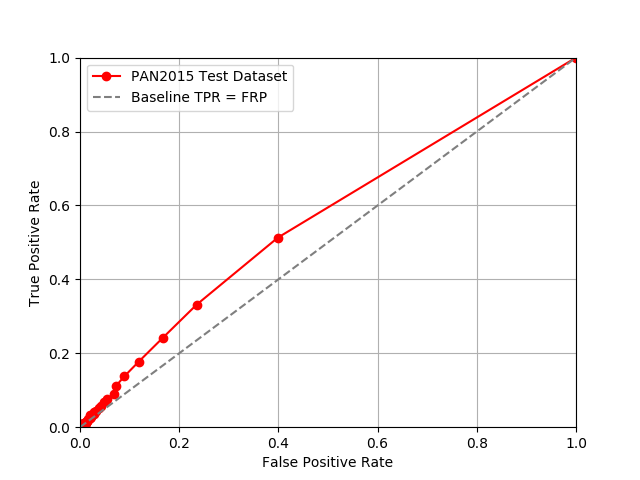
\includegraphics[width=.7\textwidth]{./pictures/delta_method_roc.png}
    \caption{The ROC curve of the delta method with number of opposing authors
    varying from 0 to 100 using the test dataset for PAN 2015.}
    \label{fig:delta_method_roc}
\end{figure}

\subsection{Generalising Random Forest} \label{subsec:results:generalising_random_forest}
In order to test the \gls{UBM} approach proposed by \cite{pacheco2015}, we start
by computing our feature set and generating our \gls{UBM} as described in
Section \ref{subsec:method:generalising_random_forest}.

The feature set and \gls{UBM}, are then encoded according to Equation
\eqref{eq:rf-encode}, and are used to train a random forest with parameters
matching the ones used in experiments. That is all parameters being set to their
default except \texttt{n\_estimators} that is set to 1000. At this point we
encode the feature set created from the test data, against the \gls{UBM}, which
is then fed to our trained random forest to get the predictions. This resulted
in an accuracy of 0.60400, \gls{TPR} of 0.63200 and \gls{TNR} of 0.57600 on the
pan 2015 dataset. On the other hand, we also chose to train our model using the
alternate subtraction encoding, which doesn't make use of the \gls{UBM}. The
subtraction encoding under-performed relative to the \gls{UBM} approach, with an
accuracy of 0.58400 a \gls{TPR} of 0.66800 and a \gls{TNR} of 0.50000.

We have generated the \gls{ROC} curve for both random forest tests. The area
under the curve was 0.63868 for the \gls{UBM} method and 0.56821 for the Minus
method. The curves is shown in Figure \ref{fig:forest_roc}. This means that the
Final Score, of the methods are the following:

\begin{align}
    \text{Final Score \gls{UBM}} &= c@1 \cdot AUROC = 0.604 \cdot 0.63868 = 0.3858  \\
    \text{Final Score Minus} &= c@1 \cdot AUROC = 0.584 \cdot 0.56821 = 0.3318
\end{align}

The curve was generated by computing the probability for each problem of the
answer being "same author". Then different thresholds for when a answer is
considered "same author" can be tried and the \gls{TPR} and \gls{FPR} can be
computed for all thresholds. In our case we tried the thresholds $\{0.0, 0.01,
\dots, 1.0\}$.

\begin{figure}
    \centering
    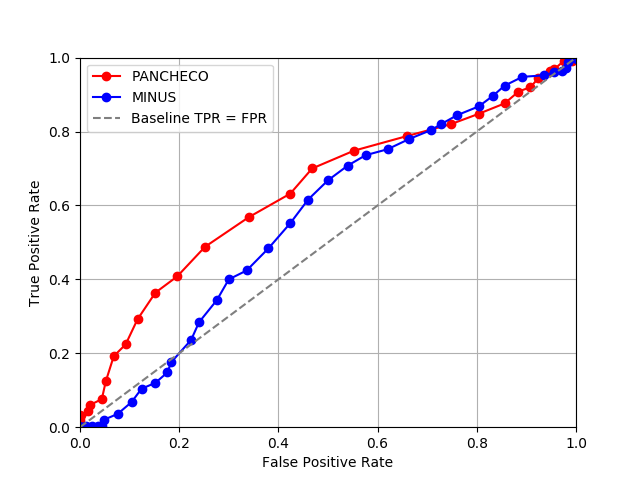
\includegraphics[width=.7\textwidth]{./pictures/forest_roc.png}
    \caption{The ROC curve of the two Generalising Random Forest
    approaches.}
    \label{fig:forest_roc}
\end{figure}

\subsection{Extended Delta} \label{subsec:results:extended_delta}
The Extended Delta Method is tested by generating features according to the best
configurations found in the training phase. Then the same procedure used to
test the regular delta method is employed. The best configuration for the PAN
2013 data were the 100 most frequent 2-, 3-, and 4-char-grams and the 300 most
frequent words for 5 opposing authors. The best configuration for the PAN 2015
data were the 20 most frequent 1-, 2-, and 3-special-char-grams for 2 opposing
authors. The accuracies, \gls{TPR}s and \gls{TNR}s obtained on all test datasets
are shown in Table \ref{tab:extended_delta_method_final_results}. The \gls{ROC}
curve is shown in Figure \ref{fig:extended_delta_method_roc} and the \gls{AUROC}
was 0.65188.

\begin{table}
    \centering
    \begin{tabular}{c|ccc}
        & \textbf{PAN 2013 Dataset 1} & \textbf{PAN 2013 Dataset 2} & \textbf{PAN 2015 Dataset} \\
        \hline
        \textbf{Accuracy}  & 0.72528 & 0.67291 & 0.61949 \\
        \textbf{\gls{TPR}} & 0.66750 & 0.75761 & 0.49760 \\
        \textbf{\gls{TNR}} & 0.77244 & 0.58953 & 0.74140
    \end{tabular}
    \caption{Result of running the extended delta method on two test sets
    included in PAN 2013 and single test set included in PAN 2015 with the best
    configurations found in the training phase.}
    \label{tab:extended_delta_method_final_results}
\end{table}

\begin{figure}
    \centering
    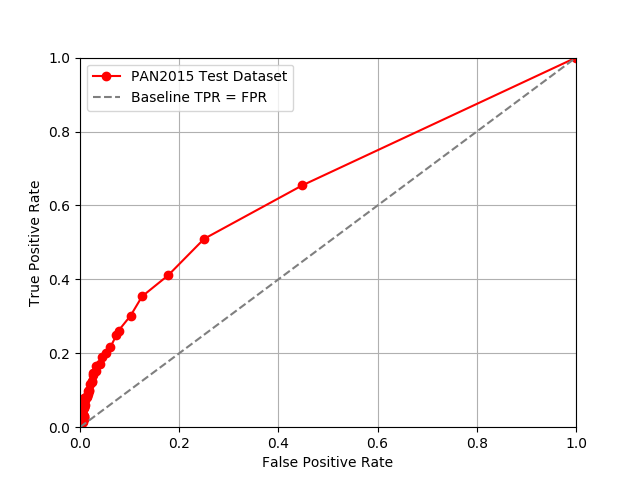
\includegraphics[width=.7\textwidth]{./pictures/extended_delta_method_roc.png}
    \caption{The ROC curve of the Extended Delta Method with number of opposing
    authors varying from 0 to 100 using the test dataset for for PAN 2015.}
    \label{fig:extended_delta_method_roc}
\end{figure}

\subsection{Author Specific SVM} \label{subsec:results:author_specific_svm}
The Author Specific SVM is tested by generating features for the training and
test datasets for the PAN 2013 texts. For each different author in the test
dataset we extract features for all their known texts and their single unknown
text. We then draw random texts from the training dataset which will serve as
opponents to the texts written by the author. Then we train an SVM using the
texts known to be written by the author and the texts from the training dataset
and predict the unknown text using that SVM.

The best configuration on the training set were configuration B using the
frequencies of the 300 most frequent words. The results on the two test datasets
are shown in Table \ref{table:svm_results}.

\begin{table}
    \centering
    \begin{tabular}{c|cc}
        & \textbf{Test Dataset 1} & \textbf{Test Dataset 2} \\
        \hline
        \textbf{Accuracy}  & 0.77650 & 0.78066 \\
        \textbf{\gls{TPR}} & 0.71444 & 0.70785 \\
        \textbf{\gls{TNR}} & 0.82727 & 0.84437
    \end{tabular}
    \caption{Results of the Author Specific SVM on the two test datasets for PAN
    2013.}
    \label{table:svm_results}
\end{table}


    \section{Discussion} \label{sec:discussion}

\subsection{Comparison to baseline approach}
Our baseline approach was the Delta Method described in Section
\ref{subsec:method:delta_method}. One of the goals of this report was finding
and implementing methods for authorship verification that could beat our
baseline method. An overview of the different methods final results can be seen
in Table \ref{tab:all_final_results}. It can be seen that we were able to beat
the baseline method both on the PAN 2013 dataset and the PAN 2015 dataset.

% TODO: Maybe elaborate on what it means that we beat the baseline methods.

\begin{table}
    \centering
    \begin{tabular}{|c|c|c|c|}
    \hline
    \textbf{Method}             & \textbf{P2013.1 F1 Score} & \textbf{P2013.2 F1 Score} & \textbf{P2015 Final Score} \\ \hline
    Delta (BASELINE)            & 0.64438                      & 0.63291                      & 0.3188                        \\ \hline
    Random Forest (\gls{UBM}) & -                            & -                            & 0.3858                        \\ \hline
    Random Forest (Minus)       & -                            & -                            & 0.3318                        \\ \hline
    Extended Delta              & 0.73213                      & 0.67173                      & 0.4053                        \\ \hline
    SVM                         & 0.77650                      & 0.78066                      & -                             \\ \hline
    \end{tabular}
    \caption{Final results for all our implemented algorithms for authorship
    verification on the datasets that apply to the method.}
    \label{tab:all_final_results}
\end{table}

\subsection{Comparison to other PAN results}

Throughout the making of this paper, several oddities occurred, which needs
addressing in order to better understand the behavior of our implemented
verification models. In in the real world, authorship-verification problems
like this are especially relevant for companies like MaCom, who operates a
website, used for submission of high-school students assignments throughout
Denmark. While both the PAN 2013, and PAN 2015 tasks aim is to implement
authorship-verification, they both represent extremes in that very area. PAN
2013, lends itself very well to author specific methods, as it contains a lot of
text for each author, but a small amount of authors, and PAN 2015 lends itself
more to the generalized approach due to the small amount of text per author. As
such, relating our method to the real world example of MaCom might give some
perspective as well. The data MaCom has, closely resembles the data from the PAN
2013 task. However, with a lot more authors and no unknown text.

Starting off with the Generalized Random Forest
\ref{subsubsec:method:generalizing_random_forest}. This method was off to a bad
start, as the paper it was based on \cite{pacheco2015} only got 6'th place in
the PAN 2015 authorship verification task, and our implementation of that same
method only ranked 9'th. \ref{subsec: Pan2015Res} The main focus of this method
however, was the way it attempted to circumvent the lack of data, associated
with each specific author, by instead learning on the know-text dataset in
its entirety. This approach, actually worked as seen in the test results. By
learning based on a \gls{UBM}, we were able to improve the results compared to
learning on the author-specific feature difference. The lack of text associated
with each author also left quite an impact in terms of what features were
relevant. After training our random forest model, it became apparent that there
was no case where word N-grams performed well, in terms of the classification.
The suspected reason for this, might be that very lack of text. The texts being
limited to about 150 words, means that there are only that many word N-grams in
the text, which limit the variety of word N-grams. However, the word-N-grams
extracted from the brown corpus, varies a lot, and as such only a few of the
word-N-grams extracted from the brown corpus are in the actual text, this only
becomes more evident as N increases due to the limited size of the texts. As
such, while the feature might very will have a high impact in some cases, we
suspect the impact will be averaged out over all the trees in the random forest.

If this \gls{UBM} method was to be applied to the MaCom data set, time
complexity would also have to analyzed in order to determine the viability of
the Generalized RF method. By only considering $\log(N)$ features in our case,
where N is the total number of features, we are able to handle large amount of
data. The time complexity of the method can be broken down into two parts. The
creating of a tree, and number of features considered. The time complexity of a
single decision tree, is $O(n \log{n})$, where n is the total number of leafs on
the tree. In our case, each tree considers $\log{N}$ features. This gives us a
final time complexity of $O(\log{N} \cdot n \log{n})$.\cite{RFTime}

While the method didn't provide any impressive results, the generalized approach
might very well be useful in the future, in case one comes across another data
sparse set. An improvement that could be done however, was to increase the
number of features fed to the random forest. Not only quantity, but also
different types of features than the ones used in this paper. This would
work since Random Forest by its' very nature selects the best features for
classification, we can at the cost of some run time, train on a much larger
feature-set and we suspect better results some might be produced.

\begin{itemize}
    \item Why did the delta method perform so much better on the training data?
    \item Comparison of our test results to the best ones in PAN 2013 and PAN
        2015.
    \item How does different methods scale to huge amounts of data?
    \item Discuss potential usage in future project based on TPR and TNR.
    \item What improvements could be made to any of the method used. RF Done
    \item Why did SVM's perform so well (https://link.springer.com/article/10.1023/A:1023824908771).
        \begin{itemize}
            \item SVM's can handle many thousands of features.
        \end{itemize}
    \item Manhattan performs better than euclidean in extended delta.
\end{itemize}


    \section{Conclusion} \label{sec:conclusion} 

We presented a collection of machine learning and distance based approaches
to the PAN 2013, and PAN 2015 tasks. We set out to beat the baseline a baseline
method, which in our case was the Delta Method, using a subset of algorithmic
approaches used on the two PAN tasks.

While we did succeed in doing so, the results produced for the two different
tasks were vastly different. This stems from the different nature of each of
the PAN tasks. While they both serve to verify if a person is indeed the author
of a specific text, the format of the data in the two tasks, results in vastly
different methods having to be used. As mentioned earlier, the PAN 2015 data-set
contains very little data. It does have a lot of data entries in the form of
authors, but each author only has 1 known text, and that texts' length has an
average word count of 460. After implementing several algorithm, it became
obvious that this data was more suited for a generalizing approach, due to the
high author count. This however contradicted the more appropriate approaches
for the 2013 set. With its numerous text per author, and its 1038 average word
count, the PAN 2013 set was more suited for approaches which made use of the
larger quantities of data the set provided. This different is showcased by the
performance of the Generalizing random forest and the SVM. The encoding used
for the random forest was used to get around the data lack of data in the 2015
set, by creating a generalizing model instead. Thus depending on the amount of
authors, instead of the amount of data. This resulted in the performance on the
2013 set, to be far inferior compared to the 2015 set. On the other hand, the
SVM bases itself on the large amount of data entries per author. If one was to
use that on the 2015 set, one would have to split the singular text for each
author up, to then get more data, thus further diluting the already sparse data
set, ending up with poor results.

One thing worth noting however, was that the importance of stop word was way 
above expectation. Looking at the feature importance graphs for the 
generalizing random forest, we can see that stop words in has
a great impact the classification. Not only that by special characters,
does as well, most likely due to the information about sentence composition it
conveys.



\begin{itemize}
    \item Answer the problem presented in the abstract
    \item Specific stop word features might have been good for performance.
    \item Generating opposing set from external source might have lead to better
        performance.
    \item The problem is much easier when more data is available.
    \item The problem changes depending on the data
    \item Were able to beat all baseline methods.
    \item Performed very well on PAN 2013 but not so well on PAN 2015.
\end{itemize}


    \section{Future Work} \label{sec:future_work}

Two of the algorithm we have implemented has only been applied to one of the
two datasets we have worked with. In particular the Random Forest approach has
only been applied to the PAN 2015 data and the \gls{SVM} approach has only been
applied to the PAN 2013 data. The main reason for that, is that the Random
Forest approach requires a single known text per author and the \gls{SVM}
approach require multiple known texts per author. It would be interesting to
apply the algorithms to the opposite datasets and look at their performance
there. We can transform the dataset with only a single known text to a dataset
with multiple by splitting the known text into a collection of known texts.
Similarly we can transform the dataset with multiple known texts to a dataset
with a single known text by concatenating the known texts. By making those two
transformations we could have run all methods on all data and found results for
all of them.

We would also like to apply our different implemented methods to larger
datasets. We have found in this assignment that having more text available per
author improves the performance of our methods. All our implemented methods
performed better on the PAN 2013 dataset than on the PAN 2015 dataset. For
example there is a Danish company, MaCom, that produce software for turning in
and managing school assignments. MaCom has a large database containing several
texts for each student and they have an interest in authorship verification.
They specifically want to verify that assignments uploaded by students match
their previous assignments and are not written by someone else. MaCom's main
requirement is a method that has a high \gls{TPR}. The reason is that they
don't want to falsely accuse anyone of not having written their own assignment,
while it doesn't matter as much if they miss some assignment that is written by
someone else. When the \gls{TPR} is high it means that there is few \gls{FN}s
and many \gls{TP}s. \gls{FN}s are as described earlier when we say a text is
written by a different author while it is actually written by the same.

Since MaCom has much data available per student their case most closely match
that of the PAN 2013 dataset. The method we implemented with the best \gls{TPR}
on the PAN 2013 dataset was our Extended Delta Method approach. So it would be
interesting to apply that approach to MaCom's dataset. The \gls{SVM} approach
also had a very promising \gls{TPR} on the training dataset so it would also be
interesting to try that.


    \nocite{*}
    \bibliographystyle{apalike}
    \bibliography{literature}

\end{document}
